\chapter{Materiales y Métodos}\label{cap:capitulo_3}

%---------------------------------------------------------------------------
\section{Materiales y métodos para la recolección de datos y análisis de la
	 población.}\label{section:Materiales y métodos para la recolección de datos y análisis de la población } 
Para el proyecto se realiza la validación de la conciencia digital sobre la navegación segura en internet en un grupo aleatorio aplicando una encuesta para la recolección de los datos que permiten validar o descartar la primera hipótesis. La encuesta busca evaluar el nivel de conocimiento sobre la navegación y seguridad en el ciberespacio en un grupo aleatorio de personas con datos básicos sobre la edad y el nivel de conocimiento en tecnología, además. Se realiza un muestreo aleatorio simple aplicado en el distrito de David cabecera, Chiriquí. \\
Las preguntas de la encuesta se orientaron a identificar el nivel de conciencia digital y conocimiento sobre  Malware, uso de métodos de seguridad y conocimiento sobre identificación de amenazas. \\
Para la selección de la muestra se consideró un subconjunto de la población finita de 96321 habitantes. Dato identificado en las estadísticas del INEC \cite{INEC}. \\
Los datos recopilados se analizarán con estadística descriptiva y permitirán validar o desechar la primera hipótesis. \\
Por lo tanto, realizando el muestreo con la población tenemos una muestra con un margen de error del 10\% como rango para reflejar la variación de los resultados de la población general, un nivel de confianza del 95\% para reflejar las actitudes más precisamente. Al calcular el tamaño de la muestra se obtiene el tamaño de 96 participantes que serán seleccionados aleatoriamente. \\
Para la escala de medición se aplican niveles de ponderación sobre las preguntas relacionadas a prácticas de seguridad online, en donde 1 es falta de conciencia y métodos de navegación segura, 2 uso medio de métodos seguros y conciencia media, 3 conocimiento de los riesgos y uso de mecanismos de seguridad.
%---------------------------------------------------------------------------
\section{Metodología y materiales para el desarrollo del modelo GPT.}\label{section:Metodología y materiales para el desarrollo del modelo GPT} 
Luego de la aplicación de la encuesta se realiza la recopilación de un conjunto de datos sobre buenas prácticas de navegación, consejos clasificados y etiquetados por categoría de amenazas en la web que luego son procesados para crear subconjuntos de entrenamiento y validación.
Para la construcción del modelo se utiliza el framework NanoGPT, esta es una solución a pequeña escala que permite reproducir modelos GPT simples y complejos entrenamientos con pocas líneas de código. \cite{Yang2020}

Para ello se realizan las etapas siguientes:
\begin{figure}[H]
	\centering % figure is centered on the page
	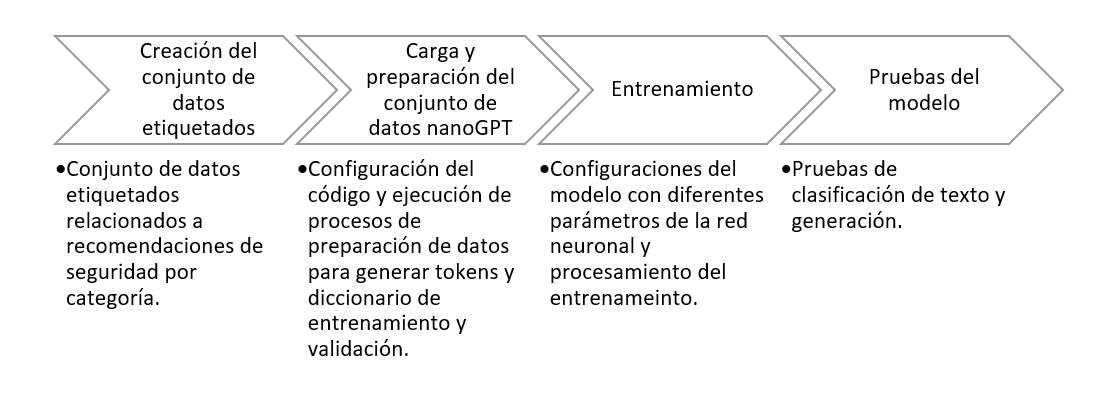
\includegraphics[width=\linewidth]{./doc/04Métodología de configuración del prototipo.png} 
	\caption{Metodología de configuración del prototipo \cite{}}
	\label{figure:Metodología de prototipado}  % assign a unique label to each figure 
\end{figure}
   
%---------------------------------------------------------------------------

%---------------------------------------------------------------------------